\documentclass[14pt]{extbook}
\usepackage{multicol, enumerate, enumitem, hyperref, color, soul, setspace, parskip, fancyhdr} %General Packages
\usepackage{amssymb, amsthm, amsmath, latexsym, units, mathtools} %Math Packages
\everymath{\displaystyle} %All math in Display Style
% Packages with additional options
\usepackage[headsep=0.5cm,headheight=12pt, left=1 in,right= 1 in,top= 1 in,bottom= 1 in]{geometry}
\usepackage[usenames,dvipsnames]{xcolor}
\usepackage{dashrule}  % Package to use the command below to create lines between items
\newcommand{\litem}[1]{\item#1\hspace*{-1cm}\rule{\textwidth}{0.4pt}}
\pagestyle{fancy}
\lhead{Progress Quiz 6}
\chead{}
\rhead{Version A}
\lfoot{4563-7456}
\cfoot{}
\rfoot{Summer C 2021}
\begin{document}

\begin{enumerate}
\litem{
First, find the equation of the line containing the two points below. Then, write the equation in the form $ y=mx+b $ and choose the intervals that contain $m$ and $b$.\[ (-4, 2) \text{ and } (-9, -2) \]\begin{enumerate}[label=\Alph*.]
\item \( m \in [0.02, 1.65] \hspace*{3mm} b \in [5.8, 6.08] \)
\item \( m \in [-1.11, 0.12] \hspace*{3mm} b \in [-9.6, -8.37] \)
\item \( m \in [0.02, 1.65] \hspace*{3mm} b \in [6.76, 7.15] \)
\item \( m \in [0.02, 1.65] \hspace*{3mm} b \in [5.11, 5.34] \)
\item \( m \in [0.02, 1.65] \hspace*{3mm} b \in [-5.6, -4.65] \)

\end{enumerate} }
\litem{
Solve the linear equation below. Then, choose the interval that contains the solution.\[ \frac{5x + 9}{6} - \frac{-7x -7}{3} = \frac{7x + 7}{4} \]\begin{enumerate}[label=\Alph*.]
\item \( x \in [1.67, 1.93] \)
\item \( x \in [-1.71, -0.62] \)
\item \( x \in [-0.54, -0.26] \)
\item \( x \in [-6.82, -5.13] \)
\item \( \text{There are no real solutions.} \)

\end{enumerate} }
\litem{
Write the equation of the line in the graph below in Standard Form $Ax+By=C$. Then, choose the intervals that contain $A, B, \text{ and } C$.
\begin{center}
    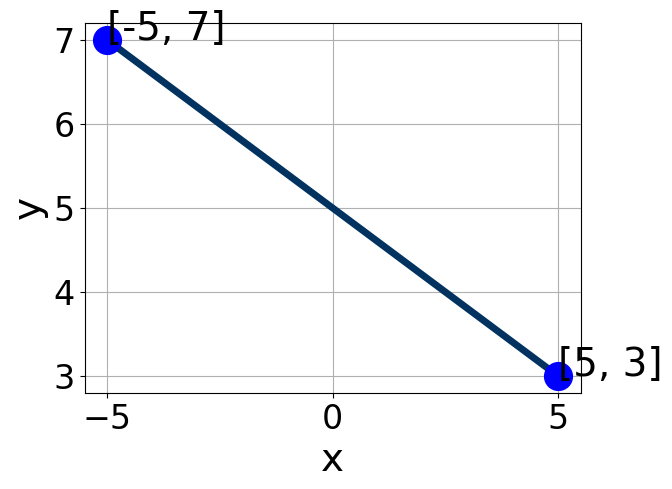
\includegraphics[width=0.5\textwidth]{../Figures/linearGraphToStandardA.png}
\end{center}
\begin{enumerate}[label=\Alph*.]
\item \( A \in [-0.6, 1.4], \hspace{3mm} B \in [-0.15, 2.2], \text{ and } \hspace{3mm} C \in [4, 9] \)
\item \( A \in [2, 9], \hspace{3mm} B \in [4.62, 5.45], \text{ and } \hspace{3mm} C \in [23, 27] \)
\item \( A \in [-0.6, 1.4], \hspace{3mm} B \in [-1.03, 0.21], \text{ and } \hspace{3mm} C \in [-5, -4] \)
\item \( A \in [2, 9], \hspace{3mm} B \in [-7.61, -3.85], \text{ and } \hspace{3mm} C \in [-30, -21] \)
\item \( A \in [-2, -1], \hspace{3mm} B \in [-7.61, -3.85], \text{ and } \hspace{3mm} C \in [-30, -21] \)

\end{enumerate} }
\litem{
Solve the equation below. Then, choose the interval that contains the solution.\[ -13(-4x -5) = -18(-19x -12) \]\begin{enumerate}[label=\Alph*.]
\item \( x \in [0.85, 1.05] \)
\item \( x \in [-0.63, -0.31] \)
\item \( x \in [-1.19, -0.82] \)
\item \( x \in [-0.8, -0.66] \)
\item \( \text{There are no real solutions.} \)

\end{enumerate} }
\litem{
Find the equation of the line described below. Write the linear equation in the form $ y=mx+b $ and choose the intervals that contain $m$ and $b$.\[ \text{Parallel to } 3 x - 8 y = 15 \text{ and passing through the point } (-3, -9). \]\begin{enumerate}[label=\Alph*.]
\item \( m \in [-0.75, 0.37] \hspace*{3mm} b \in [-10.3, -9.3] \)
\item \( m \in [0.31, 1.13] \hspace*{3mm} b \in [6.6, 10] \)
\item \( m \in [0.31, 1.13] \hspace*{3mm} b \in [-8.7, -7.1] \)
\item \( m \in [0.31, 1.13] \hspace*{3mm} b \in [-6.7, -5.4] \)
\item \( m \in [1.83, 2.85] \hspace*{3mm} b \in [-8.7, -7.1] \)

\end{enumerate} }
\litem{
Write the equation of the line in the graph below in Standard Form $Ax+By=C$. Then, choose the intervals that contain $A, B, \text{ and } C$.
\begin{center}
    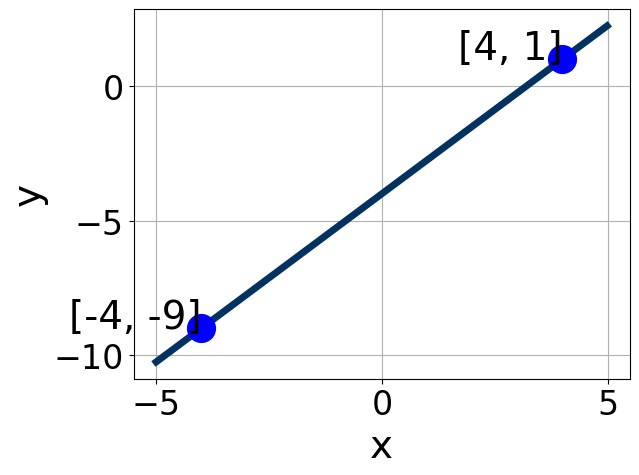
\includegraphics[width=0.5\textwidth]{../Figures/linearGraphToStandardCopyA.png}
\end{center}
\begin{enumerate}[label=\Alph*.]
\item \( A \in [2, 9], \hspace{3mm} B \in [2.7, 6.6], \text{ and } \hspace{3mm} C \in [-17, -15] \)
\item \( A \in [-8, -4], \hspace{3mm} B \in [2.7, 6.6], \text{ and } \hspace{3mm} C \in [-17, -15] \)
\item \( A \in [-4.25, 3.75], \hspace{3mm} B \in [-2.8, 0.8], \text{ and } \hspace{3mm} C \in [1, 6] \)
\item \( A \in [-4.25, 3.75], \hspace{3mm} B \in [0.1, 2.1], \text{ and } \hspace{3mm} C \in [-11, -3] \)
\item \( A \in [2, 9], \hspace{3mm} B \in [-4.2, -3.2], \text{ and } \hspace{3mm} C \in [14, 20] \)

\end{enumerate} }
\litem{
Find the equation of the line described below. Write the linear equation in the form $ y=mx+b $ and choose the intervals that contain $m$ and $b$.\[ \text{Parallel to } 4 x + 9 y = 13 \text{ and passing through the point } (5, -4). \]\begin{enumerate}[label=\Alph*.]
\item \( m \in [-0.18, 0.74] \hspace*{3mm} b \in [-6.8, -5.7] \)
\item \( m \in [-0.5, 0.02] \hspace*{3mm} b \in [-1, 4.2] \)
\item \( m \in [-0.5, 0.02] \hspace*{3mm} b \in [-12.1, -8.4] \)
\item \( m \in [-3.15, -1.79] \hspace*{3mm} b \in [-2.1, -0.3] \)
\item \( m \in [-0.5, 0.02] \hspace*{3mm} b \in [-2.1, -0.3] \)

\end{enumerate} }
\litem{
Solve the equation below. Then, choose the interval that contains the solution.\[ -2(-18x -9) = -19(-16x -8) \]\begin{enumerate}[label=\Alph*.]
\item \( x \in [-0.57, -0.33] \)
\item \( x \in [0.51, 0.65] \)
\item \( x \in [-0.97, -0.59] \)
\item \( x \in [-0.57, -0.33] \)
\item \( \text{There are no real solutions.} \)

\end{enumerate} }
\litem{
First, find the equation of the line containing the two points below. Then, write the equation in the form $ y=mx+b $ and choose the intervals that contain $m$ and $b$.\[ (-5, -9) \text{ and } (9, -2) \]\begin{enumerate}[label=\Alph*.]
\item \( m \in [0.2, 3] \hspace*{3mm} b \in [-7, -4.5] \)
\item \( m \in [-3.7, 0.4] \hspace*{3mm} b \in [-1, 3] \)
\item \( m \in [0.2, 3] \hspace*{3mm} b \in [6.1, 6.7] \)
\item \( m \in [0.2, 3] \hspace*{3mm} b \in [-12.8, -9.6] \)
\item \( m \in [0.2, 3] \hspace*{3mm} b \in [-4.6, -3.9] \)

\end{enumerate} }
\litem{
Solve the linear equation below. Then, choose the interval that contains the solution.\[ \frac{-5x -4}{2} - \frac{3x -8}{8} = \frac{-9x + 8}{4} \]\begin{enumerate}[label=\Alph*.]
\item \( x \in [-6.3, -4.5] \)
\item \( x \in [0.6, 3.2] \)
\item \( x \in [-9.5, -7.8] \)
\item \( x \in [-7.1, -6.1] \)
\item \( \text{There are no real solutions.} \)

\end{enumerate} }
\end{enumerate}

\end{document}